\documentclass[../main.tex]{subfiles}
\graphicspath{{\subfix{../images/}}}
\begin{document}
\section*{Term 2 Week 2}
\begin{enumerate}
    \item 
    \begin{figure}[H]
        \centering
        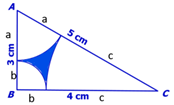
\includegraphics[width=0.25\linewidth]{images/t2w2q1_a.png}
    \end{figure}
    \(a+c=5\\
    a+b=3\\
    b+c=4\)\\
    Solving, gives \(a=2, b=1, c=3\)\\
    Area of the triangle: \(A=\frac{1}{2}\times 3 \times 4=6cm^2\)\\

    Use trigonometry to find the angles at each A, then since B = 90 we can find C. Then use these to calculate the area of each sector.\\

    \(\sin{A}=\frac{4}{5}\)\\
    \(A=\sin^{-1}{\frac{4}{5}}=53.13\)\\
    \(B=90-53.13=36.87\)\\
    Area of arc A = \(\frac{53.13}{360}\times \pi(2)^2=1.85\)\\
    Area of arc B = \(\frac{90}{360}\times \pi(1)^2=0.79\)\\
    Area of arc C = \(\frac{36.87}{360}\times \pi (3)^2=2.90\)\\
    Shaded area = \(6-1.85-0.79-2.90=0.46\)\\

    \item 
    \begin{align*}
    \frac{dV}{dt}&=kA        &   \frac{dV}{dt}&=\frac{dV}{dr}\times \frac{dr}{dt}         &  V&=\frac{4}{3}\pi r^3           &  A&=\pi r^2\\
    \end{align*}
    Combining:\\
    \(kA=4\pi r^2 \times \frac{dr}{dt}\)\\
    Therefore, \(\frac{dr}{dt}=k\)\\
    
    Separating variables and integrating:\\
    \(\int \,dr=\int k \,dt\)\\
    \(r=kt+c\)\\

    Finding initial radius and radius at time \textit{m}:\\
    \begin{align*}
    t=0, V=1      &        &t=m, V=\frac{1}{2}\\
    1=\frac{4}{3}\pi r^3   &     &\frac{1}{2}=\frac{4}{3}\pi r_m^3\\
    r=\sqrt[3]{\frac{3}{4\pi}}   &   &r_m=\sqrt[3]{\frac{3}{8\pi}}=0.49\\
    \end{align*}
    Now we can find \textit{k} and \textit{c}:\\
    When \(t=0\):\\
    \(0.62=k\times 0 + c\)\\
    \(c=0.62\)\\
    \(r=kt+0.62\)\\

    When \(t=m\):\\
    \(0.49=km+0.62\)\\
    \(km=-0.13\)\\
    \(k=-\frac{0.13}{m}\)\\

    Therefore \(r(t)=-\frac{0.13}{m}t+0.62\)\\

    When the sphere has dissolved, the radius equals zero.\\

    \(0=-\frac{0.13}{m}t+0.62\)\\
    \(\frac{0.13}{m}t=0.62\)\\
    \(t=\frac{0.62m}{0.13}=4.77m\)\\
 
    \item 
    \(f(n+2)=3^{n+3}+2^{n+2}\)\\
    Which we can rewrite as:\\
    \(3^2 \times 3^{n+1} + 2^2 \times 2^n=9\times 3^{n+1} + 4 \times 2^n\)\\

    \(f(n+1)=3^{n+2}+2^{n+1}\)\\
    Which we can rewrite as:\\
    \(3 \times 3^{n+1} + 2 \times 2^n\)\\

    Forming an equation:\\
    \(9\times 3^{n+1} + 4 \times 2^n=a(3 \times 3^{n+1} + 2 \times 2^n)+b(3^{n+1}+2^n)\)\\
    \(3 \times 3^{n+1} + 2 \times 2^n=3a \times 3^{n+1}+2a \times 2^n+b\times 3^{n+1}+b\times 2^n\)\\

    Factorising:\\
    \(9\times 3^{n+1} + 4 \times 2^n=(3a+b)3^{n+1}+(2a+b)2^n\)\\

    Therefore, we know:\\
    \(3a+b=9\)\\
    \(2a+b=4\)\\

    Solving simultaneously, we get \(a=5, b=-6\)\\
    
    \item 
    Use partial fractions to rewrite fraction:\\
    \(\frac{1}{4k^2-1}=\frac{1}{(2k-1)(2k+1)}=\frac{A}{2k-1}+\frac{B}{2k+1}\)\\

    Multiplying through by \((2k-1)(2k+1)\), we get:\\
    \(1=A(2k+1)+B(2k-1)\)\\
    \(1=2Ak+A+2Bk-B\)\\
    \(2a+2b=0 \Rightarrow a+b=0\)\\
    \(A-B=1\)\\
    \(2A=1\)\\
    \(A=\frac{1}{2}, B=-\frac{1}{2}\)\\

    So, our sum can be written as:\\
    \[\sum_{k=1}^{\infty} \frac{1}{2(2k-1)}-\frac{1}{2(2k+1)}\]\\
    
    Substitute a few values of k to see what the series looks like:\\
    \((\frac{1}{2}-\frac{1}{6})+(\frac{1}{6}-\frac{1}{10})+(\frac{1}{10}-\frac{1}{14})+...\)\\

    We can see that all the terms after the \(\frac{1}{2}\) will cancel out. This means the sum to infinity is \(\frac{1}{2}\).\\

    \item 
    Adding lines to create a series of right-angle triangles:
    \begin{figure}[H]
        \centering
        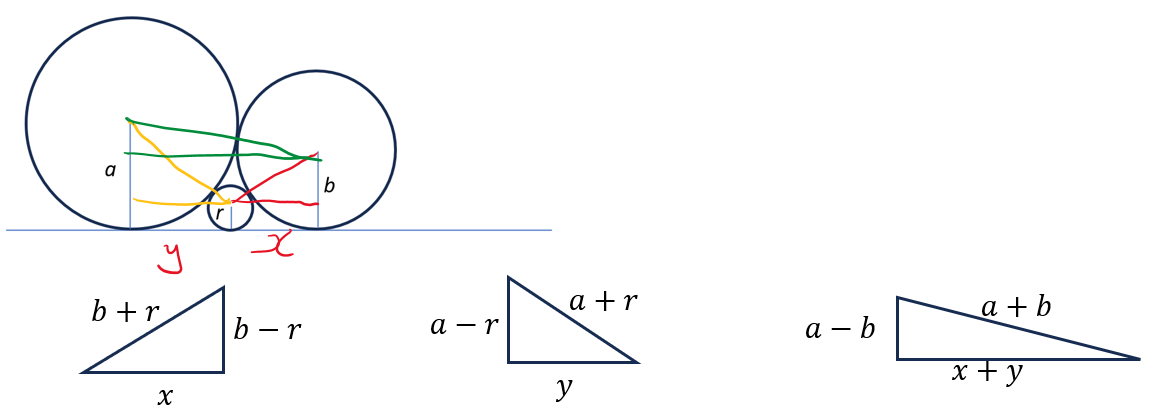
\includegraphics[width=0.75\linewidth]{images/t2w1q4_a1.png}
    \end{figure}

    Form expressions for \textit{x} and \textit{y}:\\
    \(x^2=(b+r)^2-(b-r)^2\)\\
    \(x^2=b^2+2br+r^2-b^2+2br-r^2\)\\
    \(x^2=4br\)\\
    \(x=2\sqrt{br}\)\\
    \(y^2=4ar\)\\
    \(y=2\sqrt{ar}\)\\

    \((a+b)^2=(a-b)^2+(x+y)^2\)\\
    \((a+b)^2=(a-b)^2+(2\sqrt{br}+2\sqrt{ar})^2\)\\
    \(a^2+b^2+2ab=a^2-2ab+b^2+4br+4ar+8\sqrt{abr^2}\)\\
    \(4ab=4br+4ar+8\sqrt{abr^2}\)\\
    \(ab=br+ar+2\sqrt{abr^2}\)\\
    \(ab=br+ar+2r\sqrt{ab}\)\\
    \(ab=r(a+b+2\sqrt{ab}\)\\
    \(ab=r(\sqrt{a}+\sqrt{b})^2\)\\

    Rearranging:\\
    \(\frac{1}{r}=\frac{(\sqrt{a}+\sqrt{b})^2}{ab}\)\\
    \(\frac{1}{\sqrt{r}}=\frac{\sqrt{a}+\sqrt{b}}{\sqrt{ab}}\)\\
    \(\frac{1}{\sqrt{r}}=\frac{\sqrt{a}}{\sqrt{a}\sqrt{b}}+\frac{\sqrt{b}}{\sqrt{a}\sqrt{b}}\)\\
    \(\frac{1}{\sqrt{r}}=\frac{1}{\sqrt{a}}+\frac{1}{\sqrt{b}}\)\\
    As required. 
    
\end{enumerate}

\end{document}